In this chapter, we offer an in-depth exploration of the multitude of tasks, diverse projects, and significant responsibilities that defined our enriching internship experience at NetLab!UG. These experiences spanned a wide spectrum of activities, each thoughtfully contributing to the overarching objectives of the projects while concurrently providing invaluable learning opportunities. Our narrative delves into the granular specifics of these assignments, illuminating the methodologies meticulously employed to execute them effectively.

These real-world experiences were not devoid of challenges; in fact, they presented opportunities for growth and problem-solving. Within this narrative, we candidly discuss the multifaceted challenges encountered during our tenure, offering transparency in our exploration. Furthermore, we articulate the strategic solutions devised to triumph over these hurdles, showcasing adaptability and resilience in the face of adversity.

The essence of this section lies in its ability to offer readers profound insights into the practical application of the skills and knowledge we had diligently accumulated in our academic pursuits. As we recount these endeavors, we underscore the symbiotic relationship between theoretical understanding and hands-on proficiency. Moreover, our recounting serves as a testament to the meaningful contributions we made towards the realization of key projects and initiatives within the organization.

Through this comprehensive exposition, we endeavor to convey not only the breadth and depth of our experiences but also the lasting impact of our efforts on NetLab!UG's mission and objectives. The projects undertaken were not mere tasks; they were pivotal milestones in our professional journey, offering transformative lessons and fostering a deep sense of purpose.
\section{Building Computers}

In this section, we delve into a significant project undertaken during our internship that centered on an environmentally conscious initiative: repurposing electronic waste (e-waste) obtained from MTN, a prominent telecommunications company. The project's primary objective was to salvage discarded electronic components and employ them in constructing a fully functional personal computer system. This initiative seamlessly aligns with MTN's steadfast commitment to sustainability, contributing to a reduction in electronic waste deposited in landfills and promoting the reuse of valuable resources.

\subsection{Project Overview}

The project commenced with a meticulous assessment of the collected e-waste, which included components such as motherboards, processors, memory modules, and storage devices. Our team paid careful attention to the compatibility and condition of these components, ensuring that they met the criteria for optimal performance and longevity. The construction process entailed a methodical assembly, starting from fitting the components onto the motherboard to configuring the BIOS settings for seamless operation.

\subsection{Challenges and Creative Problem-Solving}

One of the notable challenges encountered during this project was the significant variation in component specifications and interfaces. This diversity necessitated creative problem-solving to overcome compatibility issues. Collaborative efforts with colleagues and the guidance provided by our mentors proved invaluable in troubleshooting and devising effective solutions to ensure the project's success.

\subsection{Achieving Success}

The successful culmination of the project resulted in the creation of a fully functional personal computer system. This achievement served as a tangible demonstration of the feasibility of sustainable practices and the positive impact they can have on the environment. It also underscored the significance of technical skills, adaptability, and resourcefulness when addressing real-world challenges.

\subsection{Alignment with Sustainable Practices}

This project exemplifies the alignment of our efforts with broader global initiatives aimed at responsible e-waste management. It serves as a testament to the potential for positive outcomes through innovative thinking and collaborative endeavors. Our work not only showcases the practicality of repurposing e-waste but also reinforces the importance of environmentally conscious practices in today's world.

In summary, the "Building Computers" project during our internship at NetLab!UG demonstrates our commitment to sustainability, technical proficiency, and the capacity to address environmental challenges through hands-on, practical solutions.

\section{Testing E-Waste for Functional Components}

This subsection offers a detailed insight into a crucial facet of the e-waste repurposing project undertaken during our internship: the systematic and meticulous testing of collected electronic components to identify functional elements suitable for reuse. This phase of the project was instrumental in ensuring that only viable and operational parts from MTN's electronic waste inventory were integrated into the construction of the personal computer system.

\subsection{The Testing Process}

The testing phase commenced with the careful disassembly of discarded electronic devices, a process that allowed us to extract a plethora of components, including processors, memory modules, graphics cards, and storage drives. Each component, upon extraction, underwent a testing by plugging into a minimal system to confirm functionality. This process was repeated for every component, ensuring that each one was thoroughly tested and evaluated.

Components that exhibited any signs of damage, wear, or malfunction were meticulously documented and set aside for proper disposal or recycling, in strict adherence to ethical e-waste management practices. Conversely, components that unequivocally met the stringent operational standards we had set were considered prime candidates for inclusion in the personal computer assembly. Compatibility between selected components was another pivotal consideration to ensure a seamless and reliable system.

\subsection{Challenges and Adaptability}

The testing process presented its own set of challenges, primarily stemming from the remarkable variability in component types, brands, and ages found within MTN's electronic waste collection.The systems would range from the 90s Toshiba monitors to 2010's dell monitors. All ram modules ranging from DDR! through DDR4. This inherent diversity necessitated the utilization of a diverse set of testing methodologies. However, these challenges were met with a spirit of collaboration among team members and the invaluable guidance provided by experienced mentors. This collective effort proved instrumental in overcoming testing hurdles effectively and efficiently.

\subsection{Success and Implications}

The successful testing of e-waste for functional components was pivotal in ensuring the quality and reliability of the constructed personal computer system. Beyond this immediate accomplishment, this phase of the project underscored several critical lessons. It emphasized the importance of technical skills, meticulous attention to detail, and the significant role of ethical e-waste management practices in the pursuit of environmentally responsible initiatives.

In conclusion, the "Testing E-Waste for Functional Components" phase of our internship project not only contributed to the overall success of the e-waste repurposing initiative but also served as a testament to our commitment to sustainability and responsible electronics reuse. It reinforces the essential role that conscientious assessment plays in the realm of environmentally responsible practices, highlighting the broader implications of our work.




\section{Attempting PS2 Keyboard Conversion to USB Keyboard}

This section documents an informative learning experience during the internship involving the conversion of a PS2 keyboard to a USB keyboard. The primary goal was to explore the conversion process and understand the complexities involved in making legacy PS2 keyboards compatible with modern USB interfaces.

\subsection{Project Objectives}

The project's primary objectives included:

\begin{itemize}
  \item Exploring the inner workings of PS2 keyboards and their communication protocols.
  \item Investigating the feasibility of converting PS2 keyboard signals to USB signals.
  \item Identifying potential challenges and limitations in the conversion process.
\end{itemize}

\subsection{Technical Exploration}

The project began with a thorough exploration of the PS2 keyboard's internal wiring and protocol. The goal was to understand how PS2 keyboards communicate with computer systems and the unique challenges posed by their signal format.

\subsection{Conversion Attempt}

A conversion attempt was made by soldering the PS2 keyboard's D- and D+ wires to a USB connector. However, it became apparent that this straightforward approach would not suffice. The conversion process only provided power to the PS2 keyboard but did not enable it to communicate effectively with USB-enabled devices. This outcome highlighted the complexities of signal conversion and compatibility between different interfaces.

\subsection{Key Learnings}

Despite the conversion's lack of success, the project yielded valuable insights and key learnings:

\begin{itemize}
  \item Enhanced understanding of PS2 keyboard communication protocols.
  \item Recognition of the challenges in converting legacy hardware to modern interfaces.
  \item Appreciation for the intricacies of signal conversion and compatibility.
\end{itemize}

\subsection{Conclusion}

While the conversion attempt did not achieve the intended result, it was a valuable learning experience that deepened understanding of keyboard protocols and the complexities involved in interface conversions. This project emphasized the importance of careful planning and technical expertise when dealing with legacy hardware and signal conversion challenges.

\section{Building a TrueNAS Server}

This subsection shines a spotlight on a substantial project that stood out during our internship: the construction of a TrueNAS server using unconventional materials and advanced configuration techniques. The primary objective of this endeavor was to engineer a fully functional storage server within the constraints of an eco-conscious approach, involving the utilization of a cardboard case and the implementation of a robust RAID Z2 configuration to ensure data redundancy and fault tolerance.

\subsection{Project Inception}

The project's inception was marked by careful planning and resource procurement. We meticulously selected and acquired the necessary hardware components, including four hard disks and network interfaces. Notably, the unconventional choice of a cardboard case was driven by a commitment to sustainability. This aligns seamlessly with the organization's steadfast dedication to eco-friendly practices, fostering an awareness of the environmental impact of technology projects.

\subsection{Robust RAID Z2 Configuration}

The heart of the project lay in the RAID Z2 configuration, a choice that aimed to strike an ideal balance between data protection and storage capacity\cite{yi2023optimizations }. This configuration relies on two parity drives to provide a robust shield against the simultaneous failure of two disks, ensuring data integrity even in the face of challenging scenarios. The configuration process was a meticulous endeavor, involving the setup of the RAID controller and a thoughtful selection of disk drives to ensure compatibility and the attainment of optimal performance.

\subsection{Innovative Assembly and Practical Problem-Solving}

The construction phase presented unique challenges, given the unconventional cardboard case. Our innovative approach encompassed the assembly of hardware components while taking into account vital considerations such as proper ventilation and effective heat dissipation. Challenges associated with the material's limited durability and the need for creative cable management were addressed with ingenious solutions. This phase was a testament to our adaptability and practical problem-solving abilities.

\subsection{Software Setup and Rigorous Testing}

Following the successful assembly of hardware, the focus shifted to software setup. TrueNAS, a robust open-source network-attached storage (NAS) solution, was installed and configured to manage the RAID array, network connectivity, and user access permissions. Rigorous testing followed, encompassing scenarios simulating disk failures and recovery procedures, thus ensuring the server's performance, stability, and data reliability in real-world situations.

\subsection{Project Outcome and Lessons Learned}

The culmination of this project bore fruit in the form of a fully functional TrueNAS server, housed within a cardboard case. This achievement transcended mere technical prowess; it underscored the successful fusion of technical expertise with a profound sense of environmental consciousness. Moreover, it served as a powerful reminder of the versatility of unconventional materials in the realm of technology projects.

The RAID Z2 configuration, coupled with meticulous disk selection, stood as a testament to the significance of robust storage solutions in an era characterized by an ever-growing dependence on data. The project was a profound learning experience, highlighting the intrinsic value of innovative thinking, sustainability-driven practices, and the successful execution of advanced technology configurations within the constraints of eco-conscious objectives.

\section{Testing and Performance Evaluation of the TrueNAS Server}

This section delves into a crucial phase of our internship project, where we conducted thorough testing and performance evaluation of the TrueNAS server. Our goal was to ensure that the server could efficiently perform key functions, including serving as an extra storage solution for computers through Samba shares. These shares allow the server to mount as a network drive, providing additional storage to computers on the same local network.

\subsection{Assessing File Sharing Capabilities}

Our initial focus was on evaluating the server's file sharing capabilities, a fundamental aspect of data management. Specifically, we aimed to ensure that the TrueNAS server could function as extra storage for computers on the local network. To achieve this, we configured Samba shares, enabling the server to mount as a network drive on other computers. This setup facilitated seamless file sharing and provided valuable additional storage capacity to computers within the same local network.

\subsection{Virtual Machine Management}

Subsequently, we explored virtual machine management, which is crucial for efficient resource allocation and multitasking. We created a virtual environment within the server, allowing it to run multiple virtual machines (VMs) simultaneously. This capability was vital as it enabled the server to handle various tasks concurrently, similar to a chef managing multiple dishes in a busy kitchen.

\subsection{Integration of Supplementary Plugins}

To enhance the server's capabilities further, we introduced supplementary plugins. These additional tools acted as power-ups, aiding functions like file compression, security enhancements, and server performance monitoring. It was imperative that these plugins seamlessly integrated with the server without causing sluggishness or instability. While some plugins, such as Nextcloud and Plex, were tested for potential future use, they were not incorporated into the final product.

\subsection{Collaborative Problem Solving}

Throughout the testing phase, we encountered challenges that required collective problem-solving. We addressed issues such as relatively slow network connections, resource management to prevent virtual machines from overconsuming computing resources, and fine-tuning the performance of the additional plugins. Our teamwork was essential in resolving these challenges effectively.

\subsection{Validation of Success}

Upon the completion of these comprehensive tests and evaluations, we confidently assert that the TrueNAS server serves as an effective extra storage solution through its Samba shares functionality. It excels in vital functions such as file sharing, virtual machine management, and the integration of supplementary tools to enhance performance and utility. The server is poised to excel in critical tasks, acting as a dependable asset in data management endeavors.

In summary, our testing and performance evaluation confirm that the TrueNAS Server is not only reliable but also capable of serving as additional storage for computers through Samba shares. Its strong performance and versatility make it an invaluable addition to the organization's data management toolkit.

\section{Building a nextcloud server}
This subsection chronicles a significant project undertaken during the internship, focusing on the creation of a Nextcloud server using plugins within the TrueNAS CORE environment. The objective was to establish a secure and user-friendly cloud storage solution, leveraging the power of TrueNAS plugins to simplify the deployment process.

The project began with the installation of the Nextcloud plugin within the TrueNAS CORE system. The plugin, designed to encapsulate the Nextcloud application and its dependencies, streamlined the setup process and alleviated the complexities associated with manual installations. The plugin's user-friendly interface facilitated the configuration of essential parameters, such as storage location, user accounts, and access controls.

Once the Nextcloud plugin was operational, the focus shifted to integrating additional plugins to enhance the server's functionality. Plugins related to data encryption, backup, and monitoring were selected and configured to complement the core Nextcloud application. The selection process was guided by the need to strike a balance between security, performance, and user experience.

Testing constituted a pivotal phase of the project. The server's responsiveness, data synchronization across devices, and security protocols were evaluated. Collaborative efforts were invested in stress testing the system under varying loads and simulating scenarios to ensure data integrity and availability.

Challenges encountered during the project included fine-tuning plugin configurations for optimal performance, addressing compatibility issues among plugins, and ensuring a seamless user experience. These challenges were met with innovative solutions, technical expertise, and effective collaboration within the team.

The successful outcome of the project resulted in the establishment of a functional Nextcloud server within the TrueNAS CORE ecosystem. This accomplishment underscored the versatility of TrueNAS plugins in simplifying complex setups while offering a comprehensive suite of features. The integration of additional plugins enhanced the server's security, data management capabilities, and adaptability, aligning with the organization's commitment to providing robust, user-centric solutions.

\section{Configuring LAN}

This subsection outlines a pivotal aspect of the internship, detailing the setup and configuration of network infrastructure to facilitate efficient access to the NAS system through a fixed IP address. The integration of a Cisco switch, MikroTik router, and local area network (LAN) aimed to optimize connectivity, data transfer, and seamless user experience.

\subsection{Cisco Switch Configuration}

The configuration process commenced with the Cisco switch, where VLANs (Virtual LANs) were established to segregate network traffic efficiently. Ports were assigned to their respective VLANs based on device types and security requirements. Quality of Service (QoS) settings were fine-tuned to prioritize data traffic, ensuring optimal performance for critical applications.

Key steps in the Cisco switch configuration included:

\begin{itemize}
    \item Creation of VLANs: VLANs were created to logically segment the network, allowing for better control of network traffic.
    
    \item Port Assignment: Each port on the switch was assigned to a specific VLAN, ensuring that devices were placed in appropriate network segments.
    
    \item QoS Configuration: Quality of Service settings were configured to prioritize traffic based on specific criteria such as voice over IP (VoIP) or video streaming, ensuring that critical applications received sufficient bandwidth.
\end{itemize}

\subsection{MikroTik Router Configuration}

The MikroTik router configuration followed, with a focus on establishing secure and efficient routing protocols. Static routes were configured to enable seamless communication between different network segments. Firewall rules were implemented to safeguard the network against unauthorized access, while port forwarding was set up to redirect incoming traffic to the NAS system's fixed IP address.

Key steps in the MikroTik router configuration included:

\begin{itemize}
    \item Static Routing: Static routes were configured to ensure that data packets could travel efficiently between different segments of the network.
    
    \item Firewall Rules: Firewall rules were put in place to control and monitor incoming and outgoing traffic, enhancing network security.
    
    \item Port Forwarding: Port forwarding was configured to redirect external requests to the NAS system's fixed IP address, allowing remote access.
\end{itemize}

For LAN configuration, IP address assignments were managed through Dynamic Host Configuration Protocol (DHCP) to simplify device connectivity. A dedicated subnet was allocated for the NAS system, ensuring consistent communication and efficient data transfer between devices and the NAS.

The success of the configuration was gauged through thorough testing. Network connectivity, data transfer speeds, and NAS access through the fixed IP address were evaluated. Collaborative efforts among team members facilitated troubleshooting and fine-tuning of configurations.

Challenges encountered during the project included optimizing QoS settings for varying network loads, addressing IP conflicts, and ensuring seamless communication between different segments of the network. These challenges were surmounted through meticulous configuration adjustments and collaboration among team members.

The successful outcome of the project resulted in a robust network infrastructure, enabling efficient access to the NAS system through a fixed IP address. This accomplishment demonstrated the significance of effective network design and configuration in facilitating seamless data transfer, optimizing performance, and enhancing user experience.

\subsection{PoE Access Point for Lab Wi-Fi}

In addition to configuring the wired LAN infrastructure, an essential component of our network setup was the utilization of a PoE (Power over Ethernet) access point to provide seamless Wi-Fi connectivity to the lab area. This wireless solution aimed to ensure that both wired and wireless users could access network resources efficiently.

The PoE access point was strategically positioned in the lab area, taking into consideration signal strength and coverage. This access point was chosen for its ability to receive power and data through a single Ethernet cable, simplifying installation and reducing cable clutter.

Key aspects of the PoE access point setup included:

\begin{itemize}
    \item \textbf{Placement and Coverage}: The access point was strategically placed to provide optimal coverage to all lab users. Signal strength and coverage were fine-tuned to ensure a reliable Wi-Fi connection.
    
    \item \textbf{Security Configuration}: Security protocols such as WPA2-PSK (Wi-Fi Protected Access 2 - Pre-Shared Key) were implemented to safeguard the wireless network from unauthorized access.
    
    \item \textbf{Guest Network}: A separate guest network was established to allow visitors to access the internet while keeping them isolated from the internal network resources.
    
    \item \textbf{Quality of Service (QoS)}: QoS settings were applied to prioritize traffic on the wireless network, ensuring that critical applications received adequate bandwidth.
\end{itemize}

The introduction of Wi-Fi via the PoE access point significantly enhanced the flexibility and mobility of lab users. Whether working on laptops, tablets, or smartphones, all users could benefit from a fast and secure wireless connection within the lab environment.

The integration of the PoE access point seamlessly complemented the wired LAN infrastructure, providing a well-rounded networking solution for the lab. It allowed users to access network resources, including the NAS system, from both wired and wireless devices, contributing to the overall efficiency and productivity of the lab environment.
\section{Terminating Cat6 Cables}

The process of terminating Cat6 cables is a critical skill in networking and data communication installations. Proper termination ensures reliable and high-speed data transmission, making it a fundamental aspect of building robust network infrastructures. Termination involves the precise connection of connectors to Cat6 cables' twisted pairs, maintaining signal integrity and minimizing interference.

Terminating Cat6 cables follows industry-standard practices that have evolved to accommodate the demands of modern data networks. Emphasis is placed on maintaining proper cable twists within connectors to prevent signal degradation and crosstalk. Adherence to industry standards defines color codes and pin assignments for consistent terminations.

\begin{figure}[ht]
    \centering
    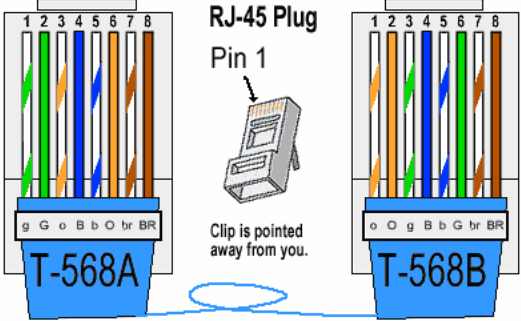
\includegraphics[width=0.6\textwidth]{images/cat6-termination.png}
    \caption{Terminating Cat6 Cable}
    \label{fig:cat6-termination}
\end{figure}

The process typically involves using a crimping tool to cut the cable and attach RJ45 connectors. These connectors securely seal off the individual wires within the cable, ensuring a reliable and secure connection. After crimping, a pair of RJ45 cable testers is employed to confirm a proper connection through the cable before connecting computers or devices to the network switch.

Terminating Cat6 cables requires specific tools and techniques to achieve optimal results. The use of high-quality cable strippers, crimpers, and testers ensures accurate terminations and efficient troubleshooting. Cable testing post-termination to verify continuity and signal quality is essential, ensuring that the cable is ready for deployment.

Moreover, the termination process necessitates attention to detail, precision, and familiarity with the Cat6 cable's structure. Stripping the cable's jacket, untwisting the pairs, aligning the conductors, and crimping the connector are sequential steps that demand meticulous execution.

In summary, the termination of Cat6 cables is a foundational skill for establishing reliable and high-performance network connections. Adherence to industry standards, utilization of proper tools, and meticulous execution, including the use of crimping tools, RJ45 connectors, and cable testers, are vital components of successful terminations that facilitate efficient data transmission and minimal signal interference.

\section{Exploring Connecting the NAS to the Internet}

This section delves into an intriguing project undertaken during the internship – the exploration of connecting the Network-Attached Storage (NAS) system to the internet. The primary objective was to investigate the feasibility, security implications, and potential benefits of making the NAS accessible remotely over the internet and create a local hosted cloud where users can access their files from anywhere.

\subsection{Project Goals}

The project's main goals included:

\begin{itemize}
  \item Assessing the technical requirements for internet connectivity of the NAS.
  \item Evaluating the security considerations associated with remote access.
  \item Exploring the advantages and use cases of having remote access to the NAS.
\end{itemize}

\subsection{Technical Exploration}

The project initiated with a comprehensive technical exploration of the NAS system and its compatibility with internet connectivity. This involved:

\begin{itemize}
  \item Examining the NAS's network capabilities and available ports.
  \item Researching secure protocols and encryption methods for remote access.
  \item Assessing the hardware and software prerequisites for internet connectivity.
\end{itemize}

\subsection{Exploring Remote Access Solutions}

Initially, we attempted to use a load balancer service from freeloadbalancer.com to forward our Nextcloud server through the internet. However, full control required a monthly subscription fee, which was not in line with our project's objectives.

Subsequently, we explored the option of DNS port forwarding over a MikroTik router to a free domain name provided by noip.com. While this approach appeared promising, we encountered technical challenges that prevented us from establishing the connection.

\subsection{Technical Challenges and Learning}

The project became a valuable learning journey about network firewalls and network administration. Challenges included:

\begin{itemize}
  \item The complexities of load balancer configurations.
  \item The technical intricacies of DNS port forwarding.
  \item The need for a deeper understanding of network security and administration.
\end{itemize}

\subsection{Outcome}

Despite the initial attempts, we ultimately decided to host the Nextcloud server locally due to the technical complexities and subscription costs associated with external services. This local setup allowed for convenient access within the organization's network, although it limited remote accessibility.

In conclusion, the project provided valuable insights into network administration, security, and remote access solutions. While we did not achieve our initial goal of connecting the NAS to the internet, the experience gained contributes to our understanding of network complexities and informs future decision-making regarding remote access solutions.

\section{3D Design of a Computer Case}

This section highlights a hands-on and creative project undertaken during the internship – the design of a computer case using two distinct software tools, Fusion 360 and Blender. The primary objective was to leverage the capabilities of both software platforms to conceptualize, model, and refine a unique computer case design that places a strong emphasis on functionality, aesthetics, and manufacturability.

\subsection{Project Initiation}

The design journey commenced with the utilization of Autodesk Fusion 360, a robust parametric modeling tool. Initial sketches and design concepts were transformed into a digital format, allowing for dynamic adjustments and iterative refinement. The parametric nature of Fusion 360 facilitated the exploration of various design elements, including dimensions, angles, and features, all while ensuring a consistent and coherent design.

\subsection{Enhancing Aesthetics in Blender}

Once the foundational design was established in Fusion 360, the project transitioned to Blender, a powerful 3D modeling and animation software. Blender's versatile toolset enabled the addition of intricate details, textures, and surface finishes that significantly contributed to the computer case's visual appeal. The non-linear workflow of Blender allowed for artistic freedom in refining the aesthetics and adding fine details to the design.

\subsection{Overcoming Challenges}

Throughout the design process, several challenges were encountered. These challenges included optimizing the design for manufacturability, ensuring proper ventilation, and maintaining structural integrity. Addressing these challenges required meticulous design adjustments, creative problem-solving, and collaborative consultation with mentors and peers.

\subsection{Iterative Refinement}

The iterative nature of the design process involved multiple rounds of feedback and refinement. Collaborative efforts were invested in critiquing and enhancing the design to meet both functional and visual objectives. The utilization of both Fusion 360 and Blender proved to be instrumental in visualizing and effectively communicating design concepts.

\subsection{Successful Outcome}

The project culminated in the creation of a comprehensive and visually appealing hexagon computer case design. The integration of Fusion 360's parametric capabilities and Blender's artistic freedom resulted in a design that elegantly balances functionality and aesthetics. This project underscores the significance of leveraging diverse software tools to transform creative visions into tangible and refined designs.

This hands-on experience in 3D design not only expanded technical skills but also provided valuable insights into the intersection of art and engineering within the context of product design.

\section{Manufacturing at Motiv}

The exploration of manufacturing practices during the internship provided valuable insights into the real-world application of innovative design and production methodologies. Manufacturing was conducted at GNEX, which is hosted at Motiv due to the availability of advanced machinery such as laser cutters, 3D printers, and woodworking machines located at Motiv.

% insert image here
\begin{figure}[H]
    \centering
    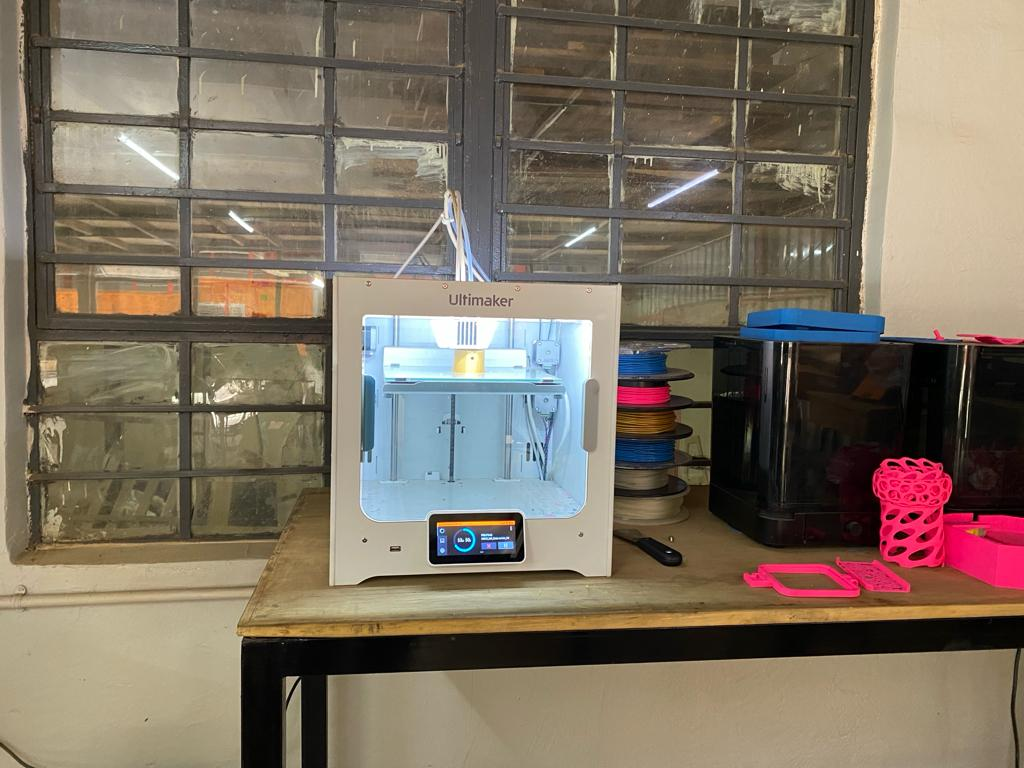
\includegraphics[width=0.8\textwidth]{images/3d-printer.jpeg}
    \caption{3D Printer at Motiv}
    \label{fig:3D Printer at Motiv}
\end{figure}


\begin{figure}[H]
    \centering
    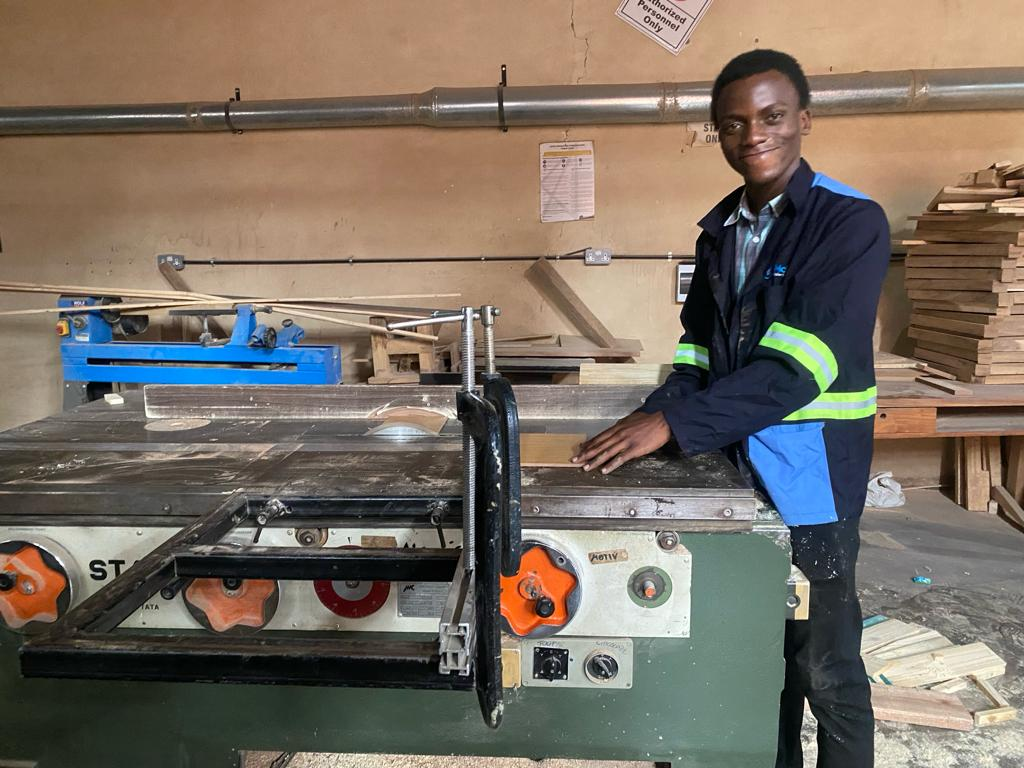
\includegraphics[width=0.8\textwidth]{images/woodPlaner.jpeg}
    \caption{Wood thickener at Motiv}
    \label{fig: Wood thickener at Motiv}
\end{figure}

Motiv, a prominent player in the technology industry, is committed to cutting-edge technology and sustainability, as exemplified by its adoption of advanced manufacturing techniques and materials. These practices align with the principles of Industry 4.0, characterized by the integration of digital technologies, automation, and data-driven decision-making into manufacturing operations. This approach streamlines production, enhances product quality, and reduces time-to-market.

Moreover, Motiv places a strong emphasis on sustainability and eco-conscious manufacturing practices, consistent with contemporary trends in corporate responsibility. By incorporating recycled and environmentally friendly materials, Motiv contributes to the reduction of carbon footprint and resource depletion.

\begin{figure}[ht]
\centering

\includegraphics[width=0.6\textwidth]{images/motiv-manufacturing.png}
\caption{Motiv's Advanced Manufacturing Facility}
\label{fig:motiv-manufacturing}
\end{figure}

Motiv's commitment to lean manufacturing principles also merits attention. The application of lean methodologies, as observed at GNEX within the Motiv premises, optimizes resource utilization, eliminates waste, and enhances overall operational efficiency.

In conclusion, an in-depth analysis of manufacturing practices at GNEX hosted at Motiv underscores the integration of technology, sustainability, and lean methodologies to drive innovation in the technology industry. The adoption of Industry 4.0 principles, eco-conscious materials, and lean manufacturing techniques positions Motiv as a trailblazer in modern manufacturing practices.

\section{Configuring a Gaming Server with Dual GPUs, Dual Motherboards, and Dual Power Supplies}

This subsection outlines a complex and technically intricate project undertaken during the internship – the configuration of a gaming server that utilizes dual GPUs, dual motherboards, and dual power supplies, all powered by a single CPU. The objective was to harness the computing power of the system to deliver optimal gaming performance and handle resource-intensive tasks.

\subsection{Project Initiation}

The project commenced with meticulous hardware selection, ensuring compatibility and performance optimization. Two high-performance GPUs were chosen to cater to the demands of modern gaming and graphics-intensive applications. Dual motherboards facilitated the management of resources and expansion possibilities, while two power supplies were implemented to distribute power efficiently. The utilization of a single CPU was a unique design choice that required creative solutions to ensure compatibility and stability.

\subsection{Configuration Process}

The configuration process involved rigorous cable management to ensure optimal airflow, thermal performance, and system stability. BIOS settings were fine-tuned to enable proper recognition of components and to maximize the utilization of resources.

\subsection{Testing and Optimization}

During the testing phase, benchmarking software and stress tests were employed to evaluate the system's stability, cooling efficiency, and gaming performance. Collaborative efforts within the team facilitated troubleshooting and optimization, ensuring that the server could deliver consistent and reliable performance.

\subsection{Challenges and Solutions}

Challenges faced during the project included running a 13-year-old CPU with a three-year-old GPU, which required creative solutions to balance performance and compatibility. Additionally, there were issues with mismatched grounds between the two motherboards, requiring meticulous electrical adjustments and grounding solutions. These challenges were addressed through a combination of technical expertise and collaborative problem-solving.

\subsection{Project Outcome}

The successful outcome of the project was the establishment of a high-performance gaming server that leveraged dual GPUs, dual motherboards, dual power supplies, and a single CPU. The configuration demonstrated the integration of cutting-edge hardware to deliver an immersive and seamless gaming experience. Additionally, the project showcased the complexity of managing resources, power, and cooling in a multi-component system.

\section{Summary}

In culmination, the internship has been a transformative and multifaceted experience that has provided a comprehensive understanding of various aspects of the field. Through a diverse array of projects, ranging from technical configurations to innovative designs, the internship has imparted invaluable skills, insights, and collaborative aptitude.

The project involving the configuration of a gaming server stands as a testament to the intricate nature of hardware integration and resource management. By configuring dual GPUs, dual motherboards, dual power supplies, and a single CPU, the project highlighted the complexities of orchestrating high-performance computing systems while optimizing power and cooling considerations. The process underscored the significance of meticulous hardware selection, fine-tuning BIOS settings, and rigorous stress testing to ensure stability and consistent performance.

The amalgamation of Autodesk Fusion 360 and Blender for the design of a computer case exhibited the dynamic interplay between parametric modeling precision and artistic expression. The creative journey of transforming initial sketches into a refined digital prototype showcased the power of iterative design, culminating in a harmonious balance between aesthetics and functionality.

Furthermore, the network configuration project involving a Cisco switch, MikroTik router, and LAN underscored the pivotal role of seamless connectivity in facilitating efficient data access to the NAS system. By meticulously configuring VLANs, routing protocols, and firewall rules, the project demonstrated the ability to create a robust and secure network infrastructure that enhances data transfer speed and accessibility.

The creation of a Nextcloud server with plugins within the TrueNAS CORE environment exemplified the significance of integrative solutions in catering to diverse user needs. The incorporation of supplementary plugins for encryption, backup, and monitoring showcased the adaptability of the system to accommodate an array of functionalities, augmenting both security and user experience.

The utilization of e-waste components for the construction of a TrueNAS server presented an innovative and sustainable approach to technology utilization. By repurposing discarded electronic components, the project embodied ethical e-waste management practices while contributing to the organization's environmental initiatives.

Collectively, these projects have cultivated a multifaceted skill set that encompasses technical prowess, creative problem-solving, collaboration, and adaptability. As the internship concludes, the gained knowledge and experiences will undoubtedly serve as the foundation for continued growth and success in the dynamic realm of technology.











